\documentclass[../AnalisideiRequisiti.tex]{subfiles}

\begin{document}
	% Il comando UserCase accetta primo una label nel caso serva un link verso di lui \refer{label} poi
	% Attore primario
	% Attore secondario
	% Descrizione
	% Precondizione
	% Postcondizione
	% Scenario principale
	% Scenari alternativi
	
	\chapter{Casi d'uso}
	\section{Classificazione dei casi d'uso}
	I casi d'uso sono identificati da un codice descritto nelle NP (§2.2.3.4).
	Di seguito viene visualizzato il diagramma generale dei casi d'uso del sistema.
	
	\section{Visione generale del sistema}
	Segue un diagramma dei casi d'uso che riassume la visione generale del sistema da sviluppare. Le sezioni successive esaminano invece i singoli casi d'uso individuati.
	
	\begin{figure}[p]
		\centering
		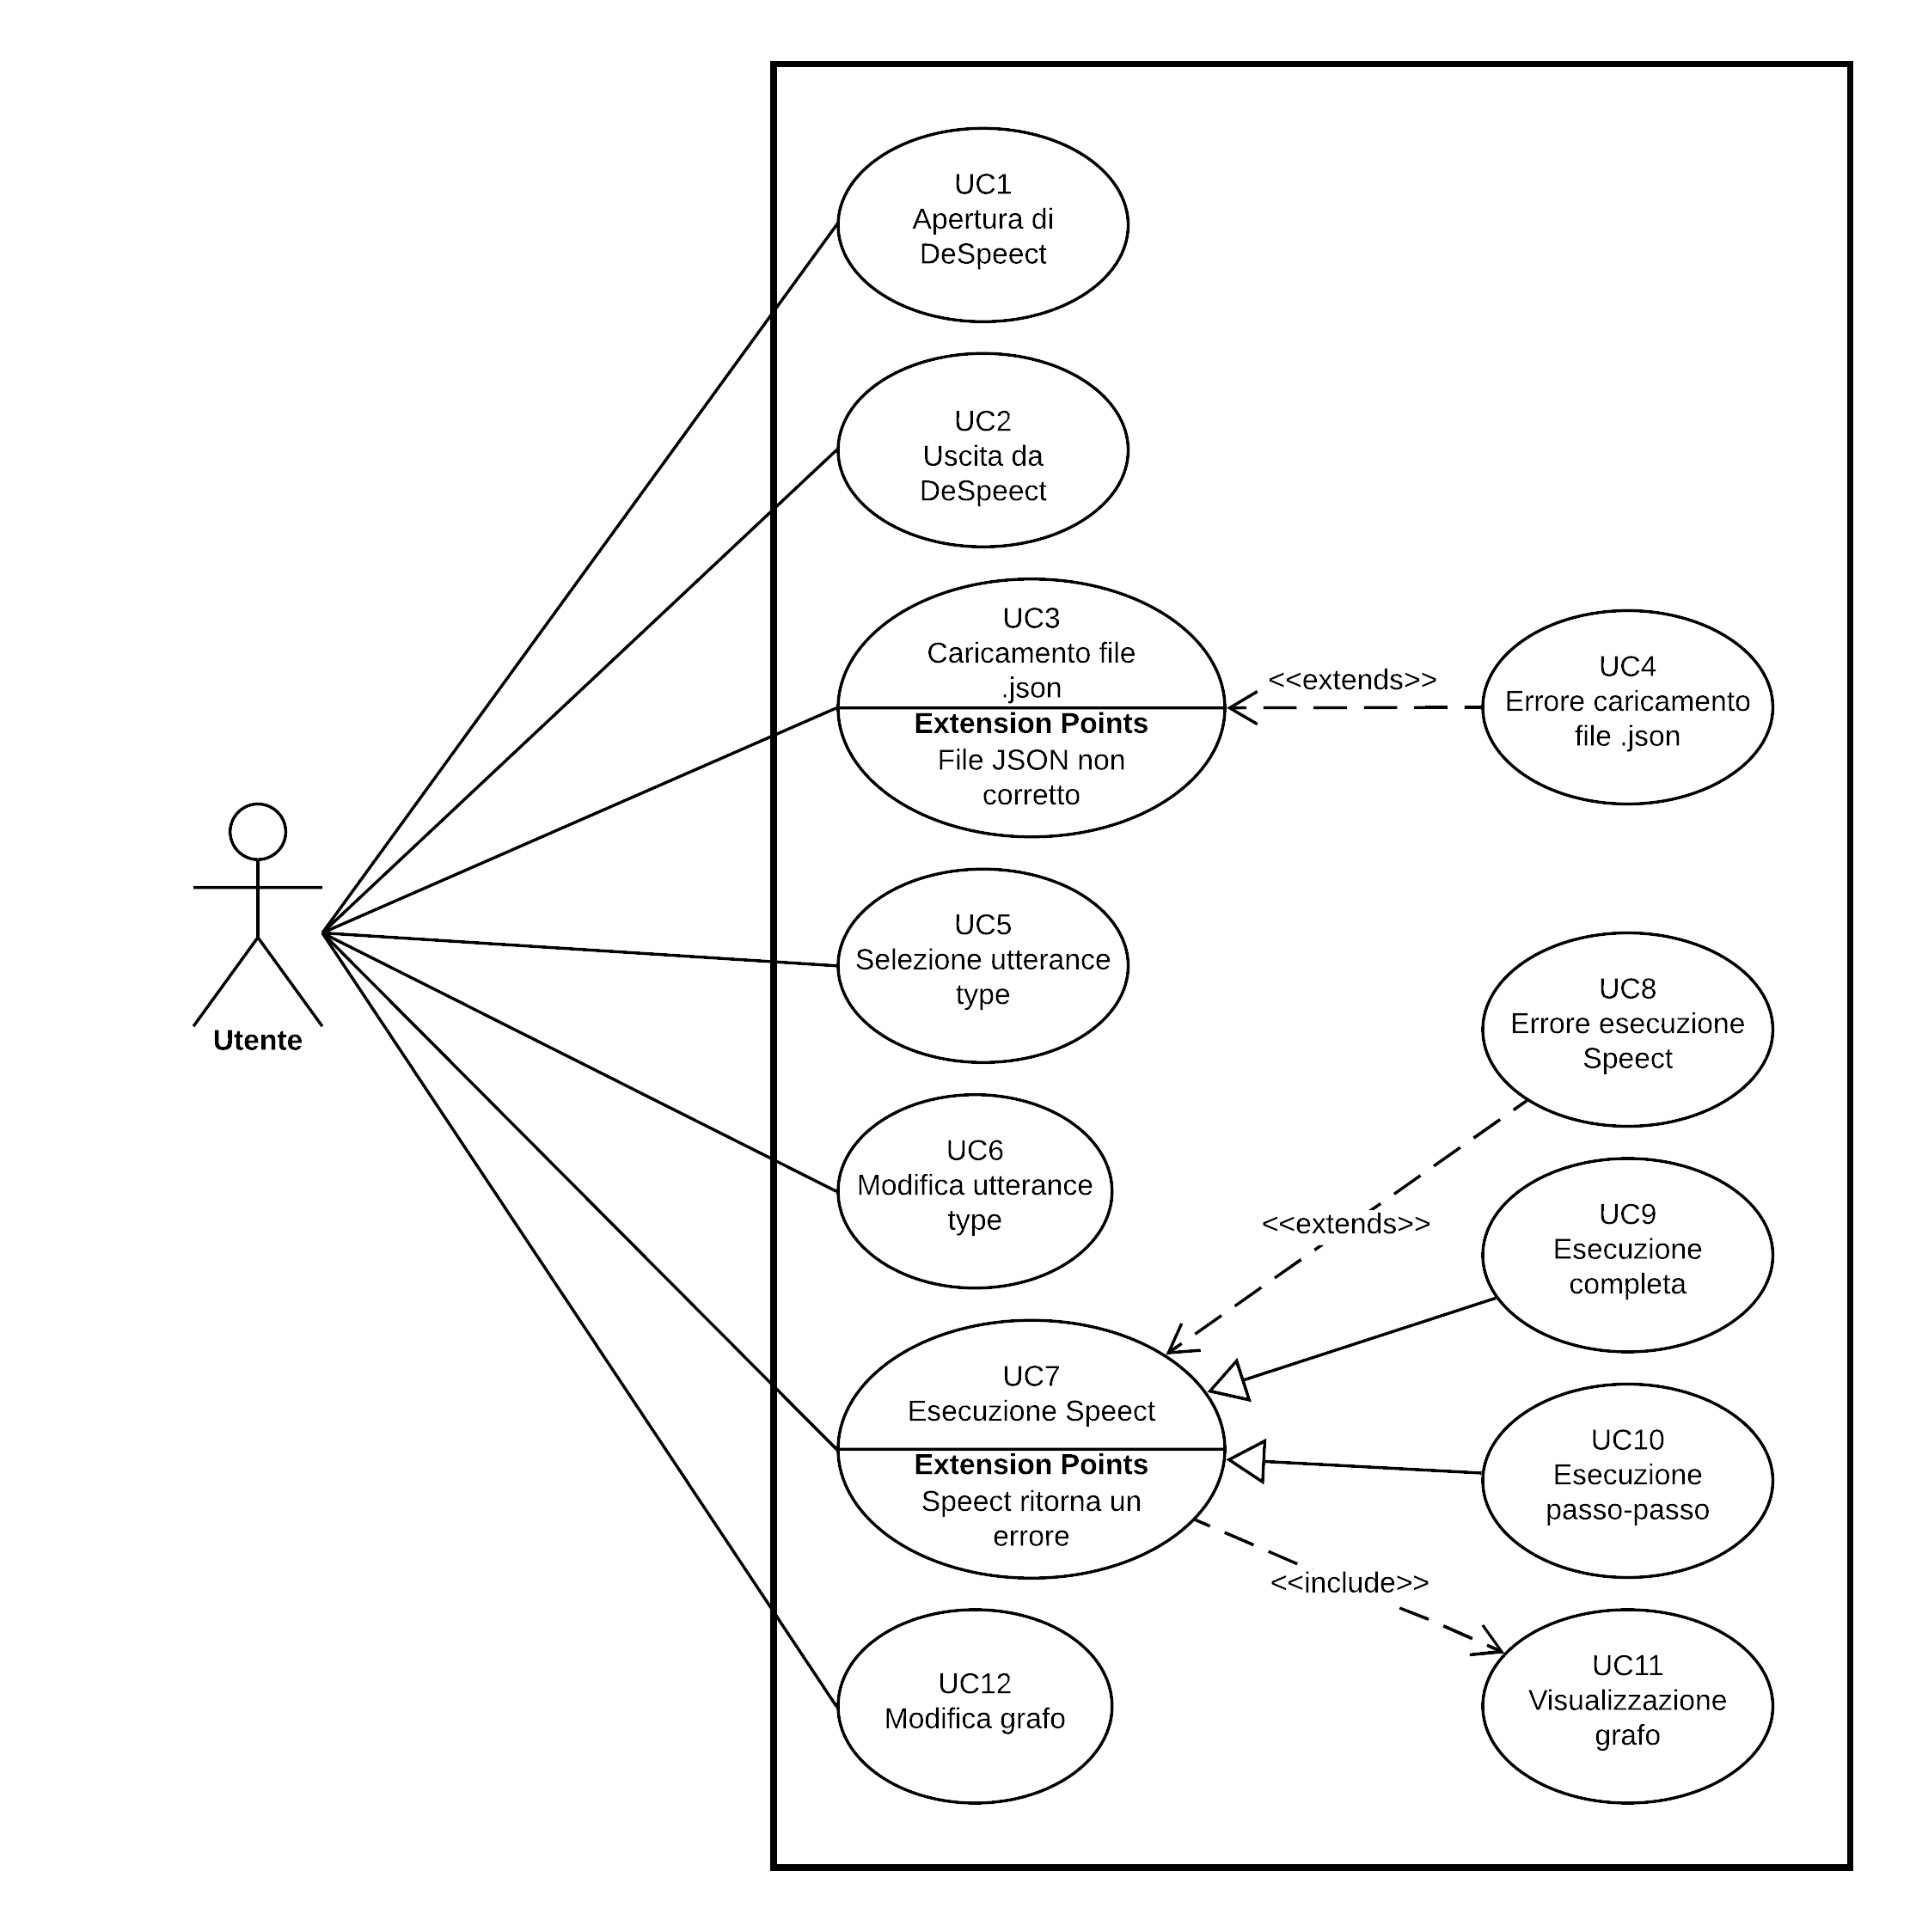
\includegraphics[width=\textwidth]{../img/UCp1.png}
		\caption{Sistema, parte 1}
	\end{figure}
	
	\begin{figure}[p]
		\centering
		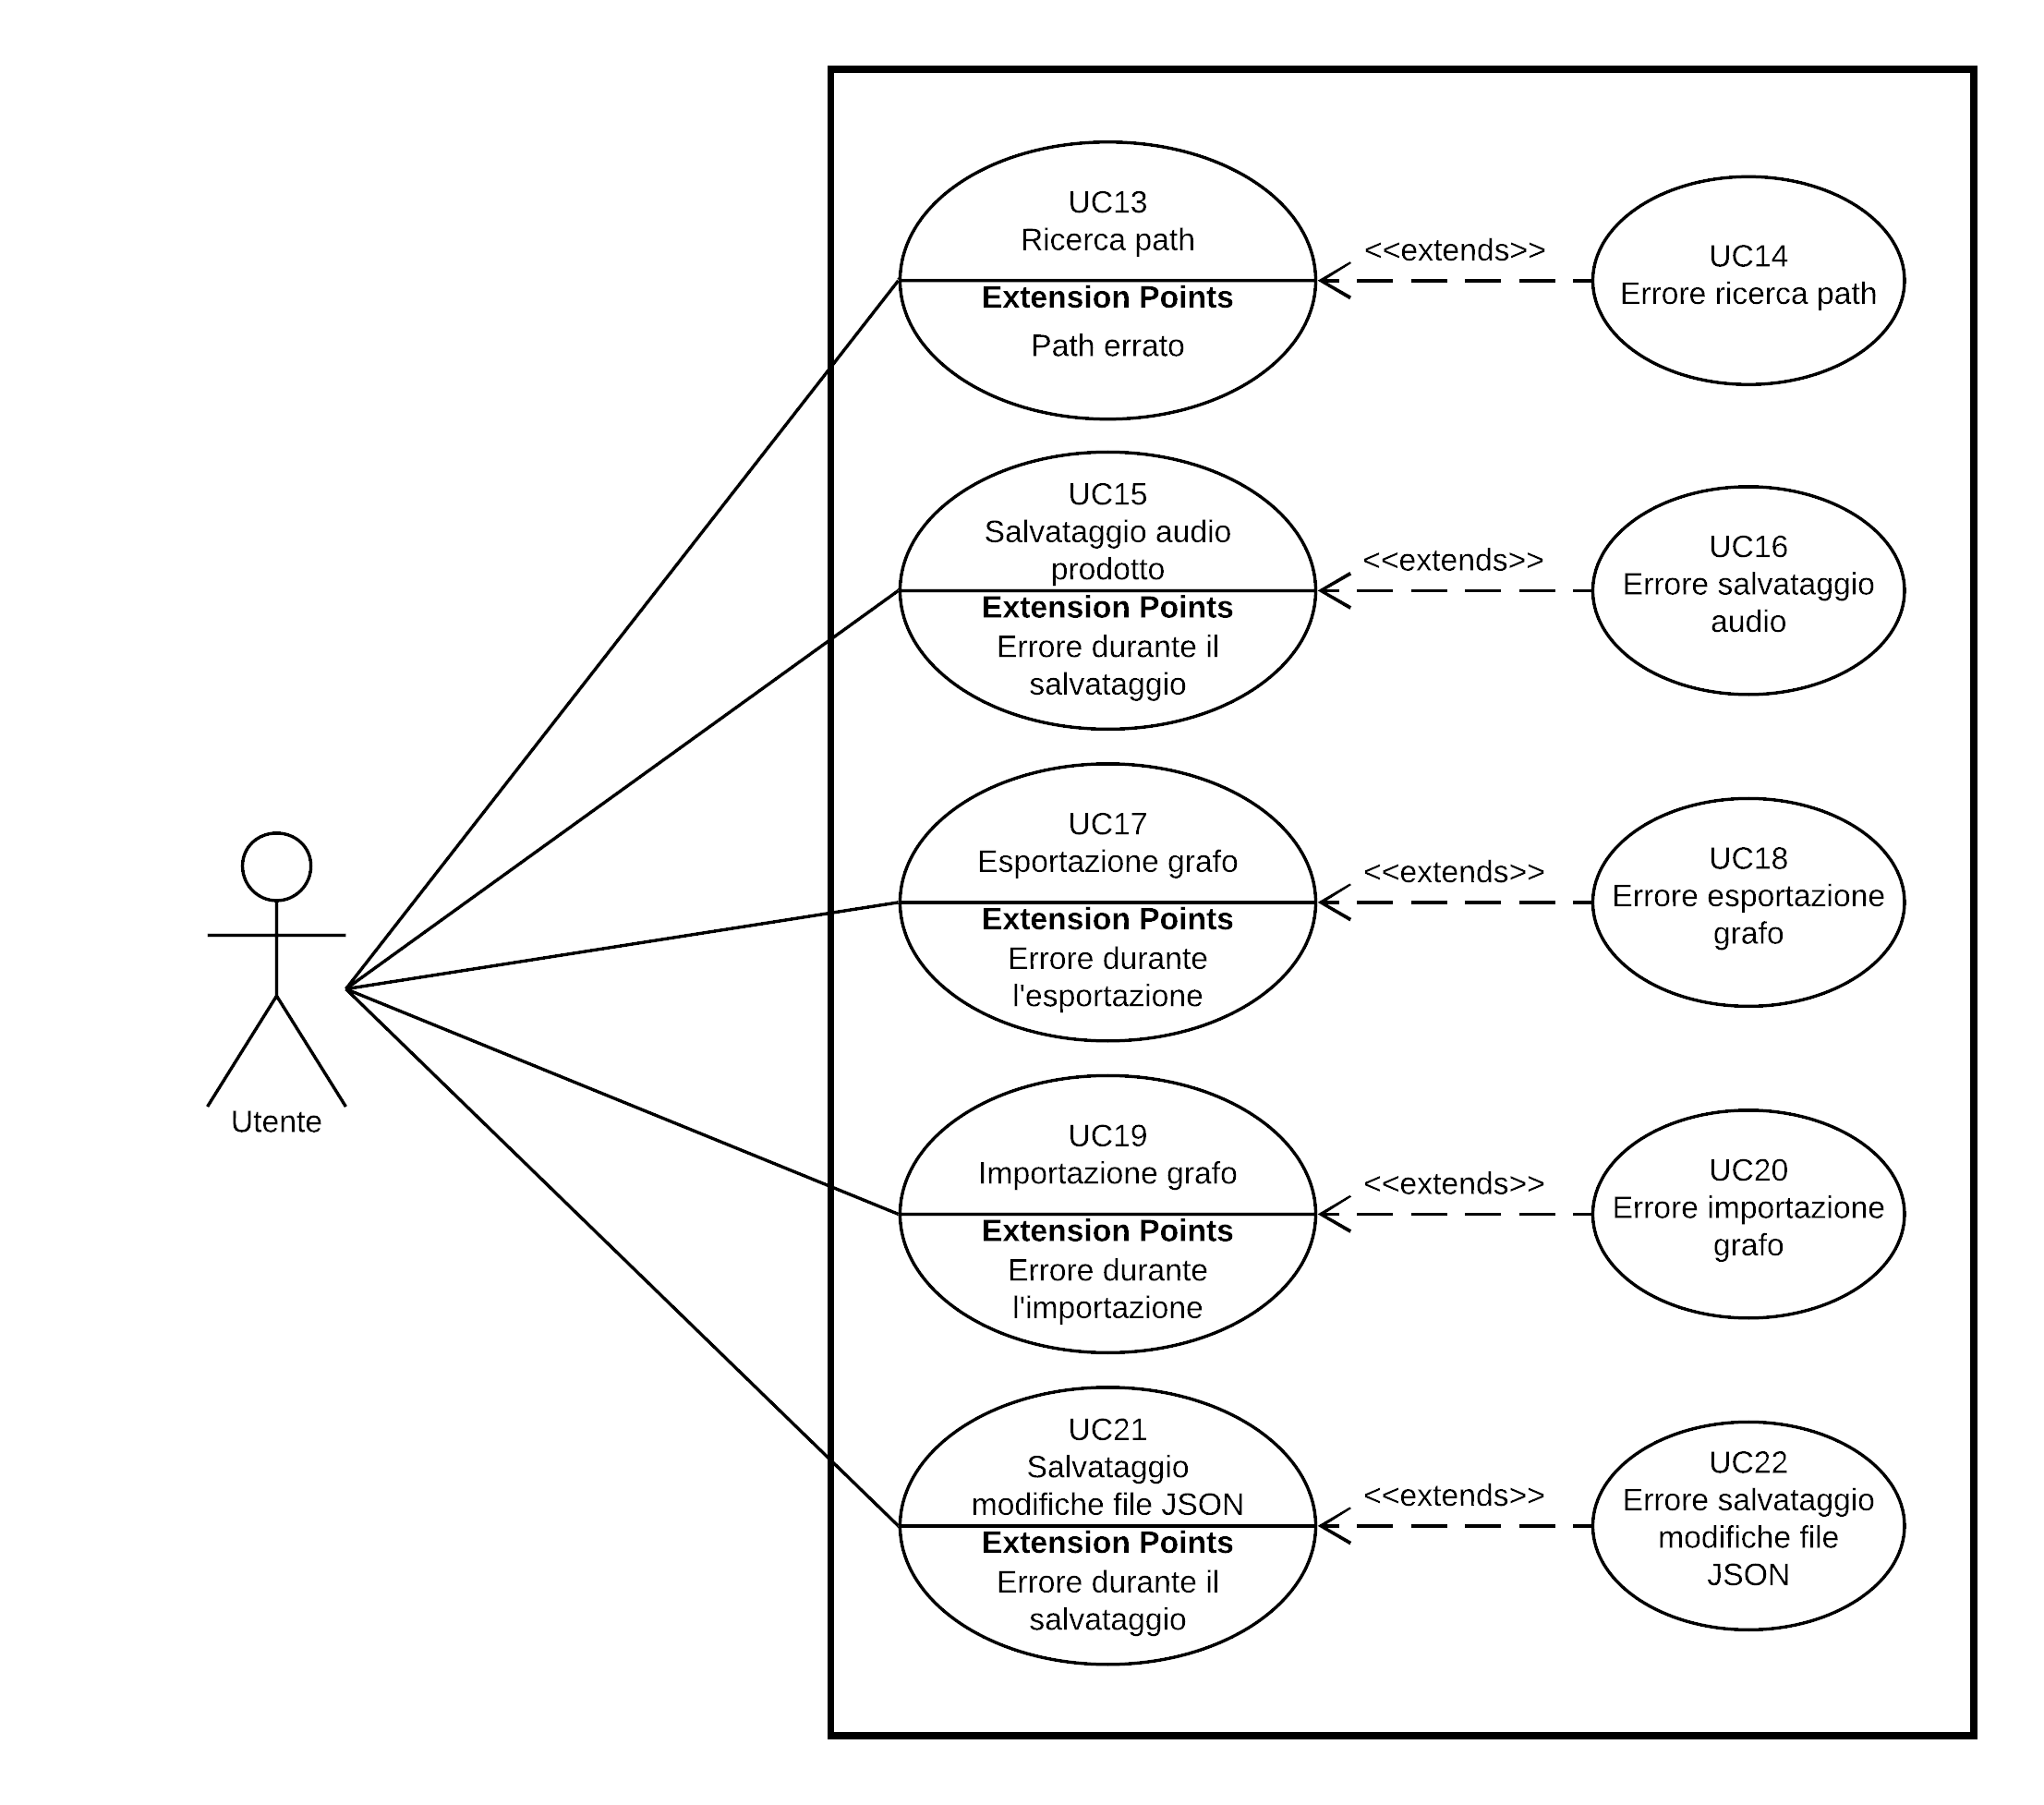
\includegraphics[width=\textwidth]{../img/UCp2.png}
		\caption{Sistema, parte 2}
	\end{figure}
	
	\section{UC1: Apertura di DeSpeect}
	\UserCase
	{UC1}
	{Utente}
	{Non previsto}
	{L'attore visualizza la pagina iniziale di DeSpeect dalla quale può caricare un file \verb|.json|, selezionare l'utterance type, modificare l'utterance type, scrivere del testo in input, eseguire Speect e modificare il grafo}
	{DeSpeect è stato avviato}
	{Viene visualizzata la pagina iniziale di DeSpeect}
	{
		\begin{itemize}
			\item{} L'attore carica un file \verb|.json| per inizializzare Speect \refer{UC3};
			\item{} L'attore seleziona una utterance type \refer{UC5};
			\item{} L'attore può modificare l'utterance type \refer{UC6};
			\item{} L'attore avvia il processo di Speect \refer{UC7};
			\item{} L'attore visualizza il grafo prodotto da Speect \refer{UC11};
			\item{} L'attore può modificare il grafo \refer{UC12}.
		\end{itemize}
	}
	{Non previsti}
	
	\section{UC2: Uscita da DeSpeect}
	\UserCase
	{UC2}
	{Utente}
	{Non previsto}
	{L'attore chiude l'applicazione}
	{L'applicazione è in esecuzione}
	{L'applicazione è chiusa}
	{Chiusura dell'applicazione}
	{Non previsti}
	
	\section{UC3: Caricamento file .json}
	\UserCase
	{UC3}
	{Utente}
	{Non previsto}
	{L'attore vuole caricare un file \verb|.json| per inizializzare Speect}
	{L'attore ha selezionato l'apposito bottone}
	{Viene inizializzato Speect con il file \verb|.json| selezionato e aggiornata la GUI}
	{
		\begin{itemize}
			\item{} Viene aperto il file browser;
			\item{} L'attore seleziona il file;
			\item{} L'attore conferma la selezione;
			\item{} Il file viene utilizzato da Speect che tenta l'inizializzazione;
			\item{} Viene visualizzato il percorso del file nell'apposito spazio \ref{fig:GUI}.
		\end{itemize}
	}
	{Speect fallisce l'inizializzazione e l'attore visualizza il messaggio d'errore relativo al file \refer{UC4}}
	
	\section{UC4: Errore caricamento file .json}
	\UserCase
	{UC4}
	{Utente}
	{Non previsto}
	{Durante l'inizializzazione, Speect fallisce ritornando un errore}
	{L'attore carica un file \verb|.json| non corretto}
	{L'errore è visualizzato, ridando controllo all'attore}
	{L'attore ha caricato un file \verb|.json| non corretto e viene visualizzato un messaggio di errore}
	{Non previsti}
	
	\section{UC5: Selezione utterance type}
	\UserCase
	{UC5}
	{Utente}
	{Non previsto}
	{L'attore vuole selezionare l'utterance type desiderata}
	{Un file \verb|.json| è stato caricato correttamente \refer{UC3}}
	{Vengono mostrati gli utterance processors utilizzati da Speect per tale utterance type}
	{
		\begin{itemize}
			\item{} L'attore apre il menu a tendina relativo;
			\item{} L'attore clicca sull'utterance type desiderata;
			\item{} Vengono mostrati a schermo i nomi degli utterance processor utilizzati, negli appositi spazi \ref{fig:GUI}.
		\end{itemize}
	}
	{Non previsti}
	
	\section{UC6: Modifica utterance type}
	\begin{figure}[H]
		\centering
		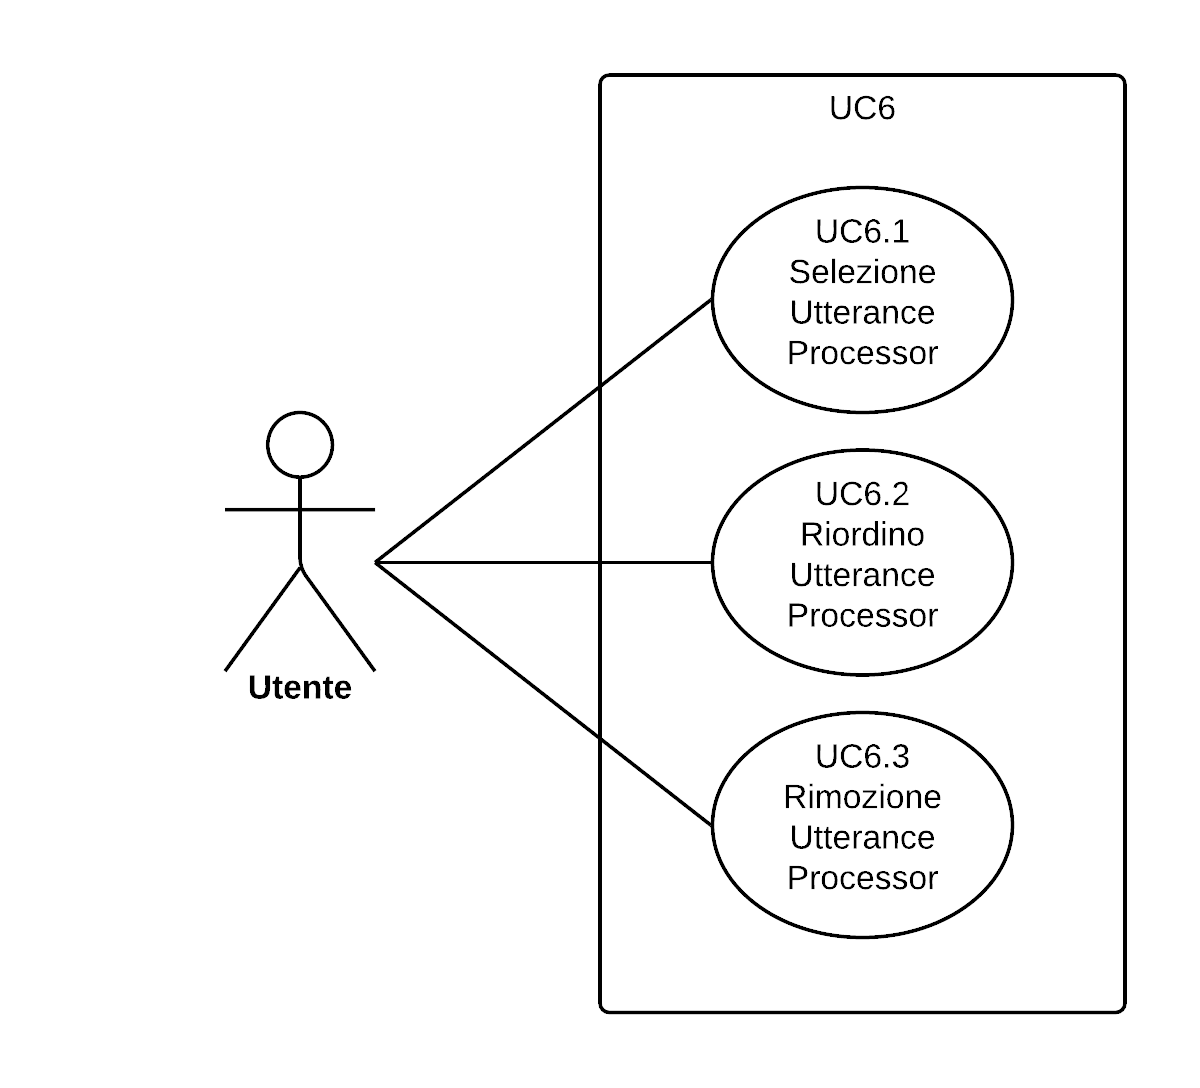
\includegraphics[width=\textwidth]{../img/UC6.png}
		\caption{UC6: Modifica utterance type}
	\end{figure}
	\UserCase
	{UC6}
	{Utente}
	{Non previsto}
	{L'attore vuole modificare l'utterance type}
	{Un file \verb|.json| è stato caricato correttamente \refer{UC3}, è presente almeno una utterance type e questa è selezionata \refer{UC5}}
	{L'utterance type è stata modificata}
	{
		\begin{itemize}
			\item{} L'attore seleziona un utterance processor;
			\item{} L'attore seleziona, riordina o deseleziona l'utterance processor;
			\item{} Le operazioni vengono eseguite.
		\end{itemize}
	}
	{Non previsti}
	
	\section{UC6.1: Selezione utterance processor}
	\UserCase
	{UC6.1}
	{Utente}
	{Non previsto}
	{L'attore vuole selezionare un utterance processor}
	{Un file \verb|.json| è stato caricato correttamente \refer{UC3}, è presente almeno una utterance type e questa è selezionata \refer{UC5}}
	{L'utterance processor è selezionato}
	{
		\begin{itemize}
			\item{} L'utterance processor è nell'elenco dei processor disponibili;
			\item{} L'attore seleziona il processor per l'esecuzione.
		\end{itemize}
	}
	{Non previsti}
	
	\section{UC6.2: Riordino utterance processor}
	\UserCase
	{UC6.2}
	{Utente}
	{Non previsto}
	{L'attore vuole cambiare l'ordine degli utterance processor}
	{L'attore ha selezionato un utterance processor \refer{UC6.1}}
	{Il file \verb|.json| viene aggiornato}
	{
		\begin{itemize}
			\item{} L'utterance processor è nell'elenco dei processor disponibili;
			\item{} L'attore modifica la posizione del processor nalla lista di esecuzione.
		\end{itemize}
	}
	{Non previsti}
	
	\section{UC6.3: Deselezione utterance processor}
	\UserCase
	{UC6.3}
	{Utente}
	{Non previsto}
	{L'attore vuole rimuovere un utterance processor}
	{L'attore ha deselezionato un utterance processor}
	{Il file \verb|.json| viene aggiornato}
	{
		\begin{itemize}
			\item{} L'utterance processor è nell'elenco dei processor disponibili;
			\item{} L'attore deseleziona il processor dalla lista di esecuzione.
		\end{itemize}
	}
	{Non previsti}
	
	\section{UC7: Esecuzione Speect}
	\UserCase
	{UC7}
	{Utente}
	{Non previsto}
	{L'attore vuole eseguire Speect}
	{Il file \verb|.json| è stato caricato correttamente \refer{UC3}}
	{Speect elabora il testo selezionato e viene visualizzato il grafo \refer{UC11}}
	{\begin{itemize}
			\item{} L'attore seleziona l'utterance type \refer{UC5};
			\item{} L'attore compila il campo di testo;
			\item{} L'attore conferma l'esecuzione;
			\item{} Vengono eseguiti gli utterance processor selezionati;
			\item{} Viene mostrato il grafo risultante dall'esecuzione \refer{UC11}.
		\end{itemize}
	}
	{Speect ha fallito l'esecuzione e l'attore visualizza un messaggio di errore \refer{UC8}}
	
	\section{UC8: Errore esecuzione Speect}
	\UserCase
	{UC8}
	{Utente}
	{Non previsto}
	{L'attore visualizza l'errore di esecuzione di Speect}
	{Speect ha fallito l'esecuzione}
	{Viene visualizzato un messaggio di errore}
	{Speect ha fallito l'esecuzione e viene visualizzato un messaggio di errore}
	{Non previsti}
	
	\section{UC9: Esecuzione completa}
	\UserCase
	{UC9}
	{Utente}
	{Non previsto}
	{Speect esegue gli utterance processors selezionati}
	{Un'utterance type è stata selezionata \refer{UC5}}
	{Vengono eseguiti gli utterance processors partendo dal grafo già presente o dal campo di testo scritto}
	{
		\begin{itemize}
			\item{} L'attore seleziona gli utterance processors desiderati \refer{UC6.1};
			\item{} L'attore può compilare il campo di testo;
			\item{} L'attore conferma l'esecuzione.
		\end{itemize}
	}
	{Speect ha fallito l'esecuzione \refer{UC8}}
	
	\section{UC10: Esecuzione passo-passo}
	\UserCase
	{UC10}
	{Utente}
	{Non previsto}
	{Speect esegue un singolo utterance processor per volta}
	{Un'utterance type è stata selezionata \refer{UC5}}
	{Viene eseguito l'utterance processor partendo dal grafo già presente o dal campo di testo scritto}
	{
		\begin{itemize}
			\item{} L'attore seleziona l'utterance processor \refer{UC5};
			\item{} L'attore può compilare il campo di testo;
			\item{} L'attore conferma l'esecuzione del singolo processor \ref{fig:GUI}.
		\end{itemize}
	}
	{Speect ha fallito l'esecuzione \refer{UC8}}
	
	\section{UC11: Visualizzazione grafo}
	\UserCase
	{UC11}
	{Utente}
	{Non previsto}
	{L'attore visualizza il grafo}
	{Speect ha terminato l'esecuzione con successo \refer{UC7}}
	{Viene visualizzato a schermo un grafo corretto con almeno un nodo cliccabile}
	{
		L'attore visualizza il grafo corretto e può modificarlo \refer{UC12}
	}
	{Non previsti}
	
	\section{UC12: Modifica grafo}
	\begin{figure}[H]
		\centering
		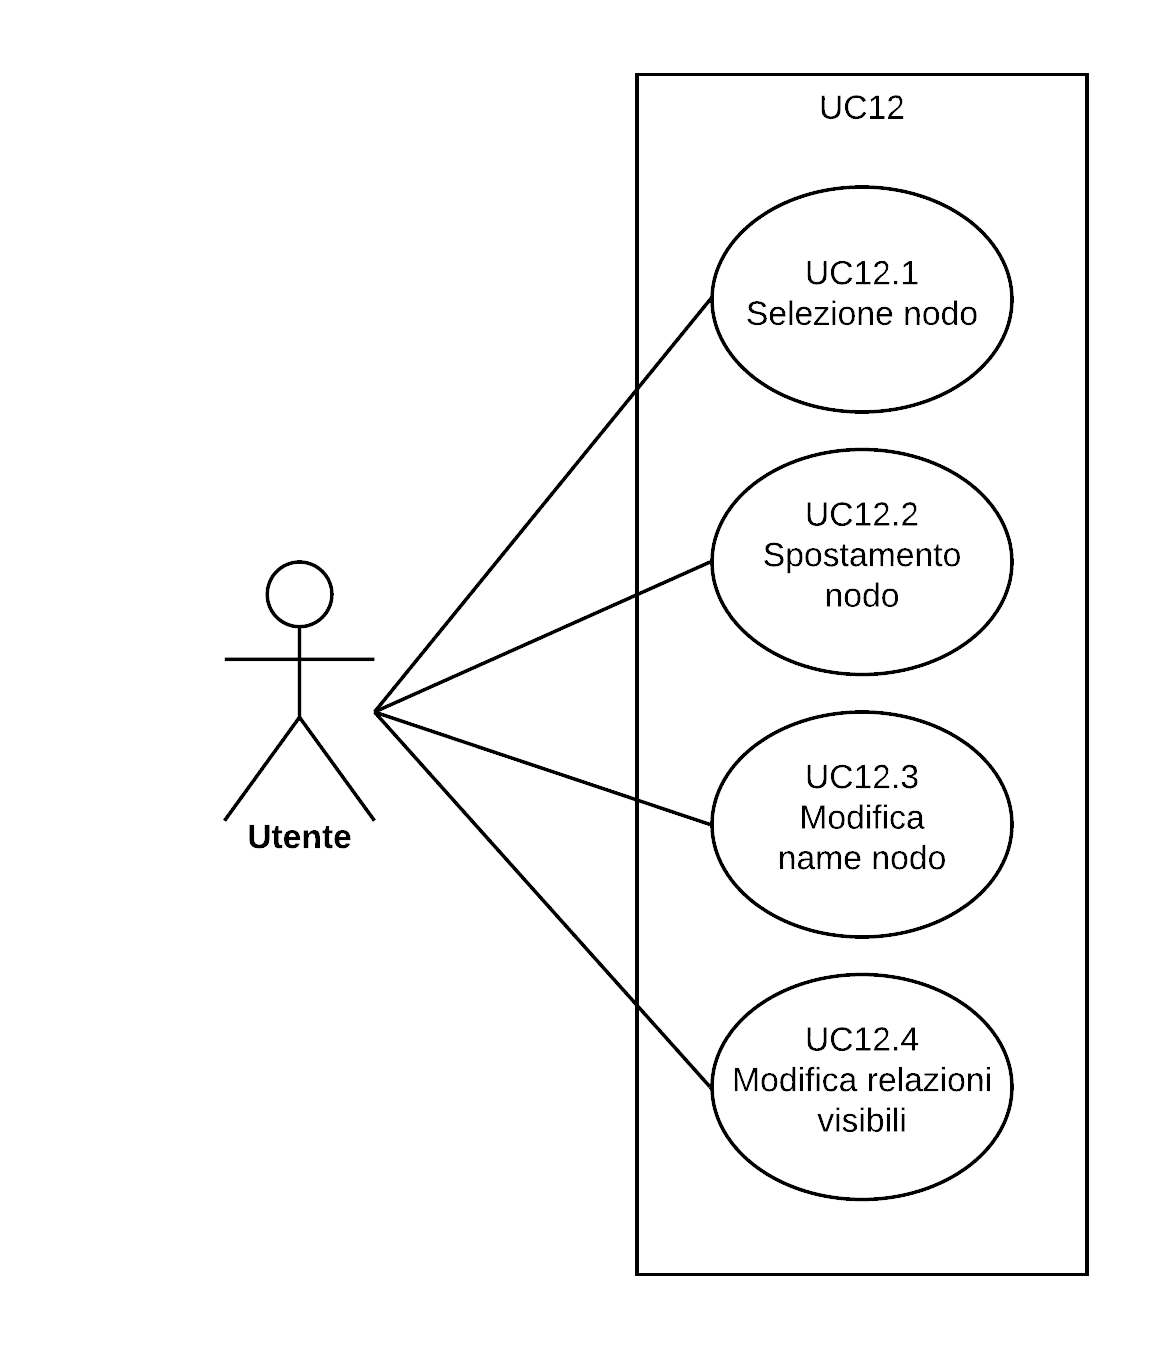
\includegraphics[width=\textwidth]{../img/UC12.png}
		\caption{UC13: Modifica grafo}
	\end{figure}
	\UserCase
	{UC12}
	{Utente}
	{Non previsto}
	{L'attore vuole modificare il grafo prodotto durante l'esecuzione di Speect \refer{UC7}}
	{Viene visualizzato a schermo un grafo corretto con almeno un nodo cliccabile \refer{UC11}}
	{Il grafo è stato modificato}
	{
		L'attore per modificare un grafo può:
		\begin{itemize}
			\item{} selezionare un nodo \refer{UC12.1};
			\item{} spostare un nodo \refer{UC12.2};
			\item{} modificare un nodo \refer{UC12.3};
			\item{} modificare la visualizzazione delle relazioni \refer{UC12.4}.
		\end{itemize}
	}
	{Non previsti}
	
	\section{UC12.1: Selezione nodo}
	\UserCase
	{UC12.1}
	{Utente}
	{Non previsto}
	{L'attore vuole selezionare un nodo per visualizzarne i dettagli}
	{Viene visualizzato a schermo un grafo corretto con almeno un nodo cliccabile \refer{UC11}}
	{Viene evidenziato il nodo del grafo e vengono mostrate le sue informazioni nella parte della GUI dedicata (\ref{fig:GUI})}
	{
		\begin{itemize}
			\item{} L'attore clicca una volta sul nodo;
			\item{} Il nodo viene evidenziato;
			\item{} Nel riquadro apposito (\ref{fig:GUI}) vengono visualizzati i dati del nodo;
			\item{} L'attore può modificare i campi del nodo selezionato \refer{UC12.3}.
		\end{itemize}
	}
	{Non previsti}
	
	\section{UC12.2: Spostamento nodo}
	\UserCase
	{UC12.2}
	{Utente}
	{Non previsto}
	{L'attore vuole spostare graficamente uno nodo o più nodi}
	{Almeno un nodo è selezionato \refer{UC12.1}}
	{I nodi selezionati vengono spostati}
	{
		\begin{itemize}
			\item{} L'attore seleziona un nodo o più nodi;
			\item{} L'attore muove i nodi;
			\item{} Il nodo rimane nella nuova posizione.
		\end{itemize}
	}
	{Non previsti}
	
	\section{UC12.3: Modifica nodo}
	\UserCase
	{UC12.3}
	{Utente}
	{Non previsto}
	{L'attore vuole modificare il name del nodo selezionato}
	{Viene visualizzato a schermo un grafo corretto con almeno un nodo cliccabile \refer{UC11}}
	{Il contenuto del nodo viene modificato}
	{
		\begin{itemize}
			\item{} L'attore seleziona il nodo \refer{UC12.1};
			\item{} L'attore modifica un campo;
			\item{} L'attore conferma la modifica;
			\item{} Il grafo viene aggiornato \refer{UC11}.
		\end{itemize}
	}
	{Non previsti}
	
	\section{UC12.4: Modifica relazioni visibili}
	\UserCase
	{UC12.4}
	{Utente}
	{Non previsto}
	{L'attore vuole filtrare le relazioni visibili del grafo}
	{Viene visualizzato a schermo un grafo corretto con almeno un nodo cliccabile \refer{UC11}}
	{Vengono mostrate nel grafo tutte le relazioni selezionate}
	{
		\begin{itemize}
			\item{} L'attore seleziona o deseleziona una relazione dalla lista delle relazioni;
			\item{} Viene adeguata la visibilità della relazione;
			\item{} Il grafo viene aggiornato \refer{UC11}.
		\end{itemize}
	}
	{Non previsti}
	
	\section{UC13: Ricerca path}
	\UserCase
	{UC13}
	{Utente}
	{Non previsto}
	{L'attore vuole cercare un nodo tramite un percorso nel grafo}
	{Viene visualizzato a schermo un grafo corretto con almeno un nodo cliccabile \refer{UC11}}
	{Viene evidenziato il nodo al termine del path}
	{
		\begin{itemize}
			\item{} L'attore seleziona un nodo \refer{UC12.1};
			\item{} L'attore inserisce il percorso da cercare;
			\item{} L'attore conferma la ricerca;
			\item{} Il nodo di arrivo viene evidenziato.
		\end{itemize}
	}
	{Il percorso inserito dall'attore non è corretto e viene visualizzato un errore \refer{UC14}}
	
	\section{UC14: Errore ricerca path}
	\UserCase
	{UC14}
	{Utente}
	{Non previsto}
	{L'attore vuole cercare un nodo tramite un percorso nel grafo}
	{Il percorso inserito dall'attore è sintatticamente errato}
	{Viene visualizzato l'errore di ricerca fallita}
	{Il percorso inserito dall'attore non è corretto e viene visualizzato un messaggio di errore}
	{Non previsti}
	
	\section{UC15: Salvataggio audio prodotto}
	\UserCase
	{UC15}
	{Utente}
	{Non previsto}
	{L'attore vuole salvare l'audio prodotto}
	{Speect è inizializzato \refer{UC3}}
	{L'audio è salvato in un file}
	{
		\begin{itemize}
			\item{} L'attore esegue Speect \refer{UC7};
			\item{} L'attore sceglie il dove salvare il file audio;
			\item{} L'attore sceglie l'estensione del file audio da generare tra i disponibili;
			\item{} L'attore scrive il nome del file nella barra di testo dedicata;
			\item{} L'attore conferma il salvataggio;
			\item{} Il file viene salvato nella destinazione con l'estensione scelta.
		\end{itemize}
	}
	{Avviene un errore durante il salvataggio dell'audio \refer{UC16}}
	
	\section{UC16: Errore salvataggio audio}
	\UserCase
	{UC16}
	{Utente}
	{Non previsto}
	{Avviene un errore durante il salvataggio dell'audio}
	{L'attore ha provato a salvare un file audio}
	{Viene visualizzato l'errore e nessun file viene generato}
	{L'attore ha cercato di salvare il file audio prodotto e viene visualizzato un messaggio di errore}
	{Non previsti}
	
	\section{UC17: Esportazione grafo}
	\UserCase
	{UC17}
	{Utente}
	{Non previsto}
	{L'attore vuole esportare il grafo visualizzato}
	{Viene visualizzato a schermo un grafo corretto con almeno un nodo cliccabile \refer{UC11}}
	{Il grafo viene esportato in un file}
	{
		\begin{itemize}
			\item{} L'attore sceglie il dove salvare il file contenente il grafo;
			\item{} L'attore scrive il nome del file nella barra di testo dedicata;
			\item{} L'attore conferma il salvataggio.
		\end{itemize}
	}
	{L'esportazione fallisce \refer{UC18}}
	
	\section{UC18: Errore esportazione grafo}
	\UserCase
	{UC18}
	{Utente}
	{Non previsto}
	{Avviene un errore durante l'esportazione}
	{L'esportazione del grafo è fallita}
	{Viene visualizzato l'errore e nessun file viene generato}
	{L'esportazione del grafo è fallita e viene visualizzato un messaggio di errore}
	{Non previsti}
	
	\section{UC19: Importazione grafo}
	\UserCase
	{UC19}
	{Utente}
	{Non previsto}
	{L'attore vuole importare un grafo come stato nell'applicazione}
	{Esiste un file contenente un grafo}
	{Il grafo viene importato da file}
	{
		\begin{itemize}
			\item{} L'attore seleziona il file da importare;
			\item{} L'attore conferma l'apertura del file.
		\end{itemize}
	}
	{L'importazione fallisce \refer{UC20}}
	
	\section{UC20: Errore importazione grafo}
	\UserCase
	{UC20}
	{Utente}
	{Non previsto}
	{Avviene un errore durante l'importazione}
	{L'importazione del grafo è fallita}
	{Viene visualizzato l'errore e nessuna operazione viene eseguita}
	{L'importazione del grafo è fallita e viene visualizzato un messaggio di errore}
	{Non previsti}
	
	\section{UC21: Salvataggio file .json}
	\UserCase
	{UC21}
	{Utente}
	{Non previsto}
	{L'attore ha modificato gli utterance processor e vuole salvare il nuovo file \verb|.json|}
	{Esiste un file \verb|.json| correttamente caricato \refer{UC3} e l'attore ha modificato gli utterance processor \refer{UC6}}
	{Le modifiche vengono salvate}
	{
		\begin{itemize}
			\item{} L'attore sceglie il dove salvare il file \verb|.json|;
			\item{} L'attore scrive il nome del file nella barra di testo dedicata;
			\item{} L'attore conferma il salvataggio.
		\end{itemize}
	}
	{L'operazione di salvataggio fallisce \refer{UC22}}
	
	\section{UC22: Errore salvataggio file .json}
	\UserCase
	{UC22}
	{Utente}
	{Non previsto}
	{L'attore ha provato a salvare il file \verb|.json|}
	{L'operazione di salvataggio fallisce}
	{Viene visualizzato l'errore e nessun file viene generato}
	{L'operazione di salvataggio fallisce e viene visualizzato un errore}
	{Non previsti}
	
\end{document}
